\newpage
\section{Anhang}
\subsection{Absorbtionsspektren}
Gezeigt sind die Absorbtionspektren der einzelnen Absorbermaterialien.
Über die gemessenen Bragg-Winkel $\Theta$ können diese nach Gl. \ref{eqn:bragg}
in die Wellenlänge und somit in die Enrgie umgerechnet werden. Der plötzliche Anstieg
im Spektrumsverlauf makiert dabei die K-Kante.
\begin{figure}[H]
    \centering
    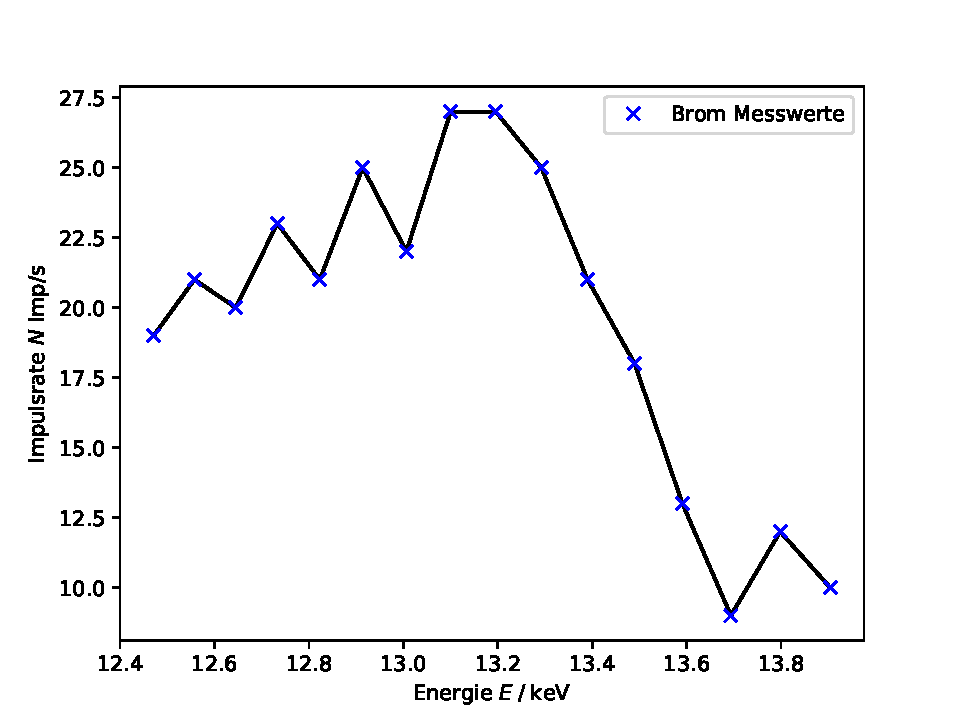
\includegraphics[width=0.7\textwidth]{plots/Brom.pdf}
    \caption{In der Abbildung ist das Absorbtionspektrum eines Bromabsorbers dargestellt}
\end{figure}
\begin{figure}[H]
    \centering
    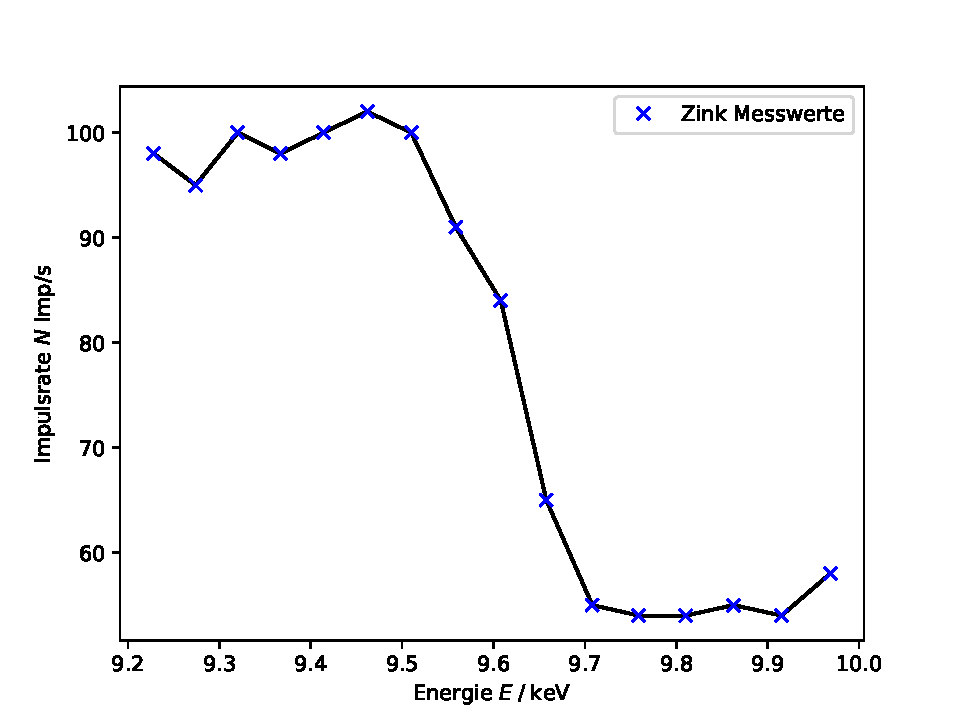
\includegraphics[width=0.7\textwidth]{plots/Zink.pdf}
    \caption{In der Abbildung ist das Absorbtionspektrum eines Zinkabsorbers dargestellt}
\end{figure}
\begin{figure}[H]
    \centering
    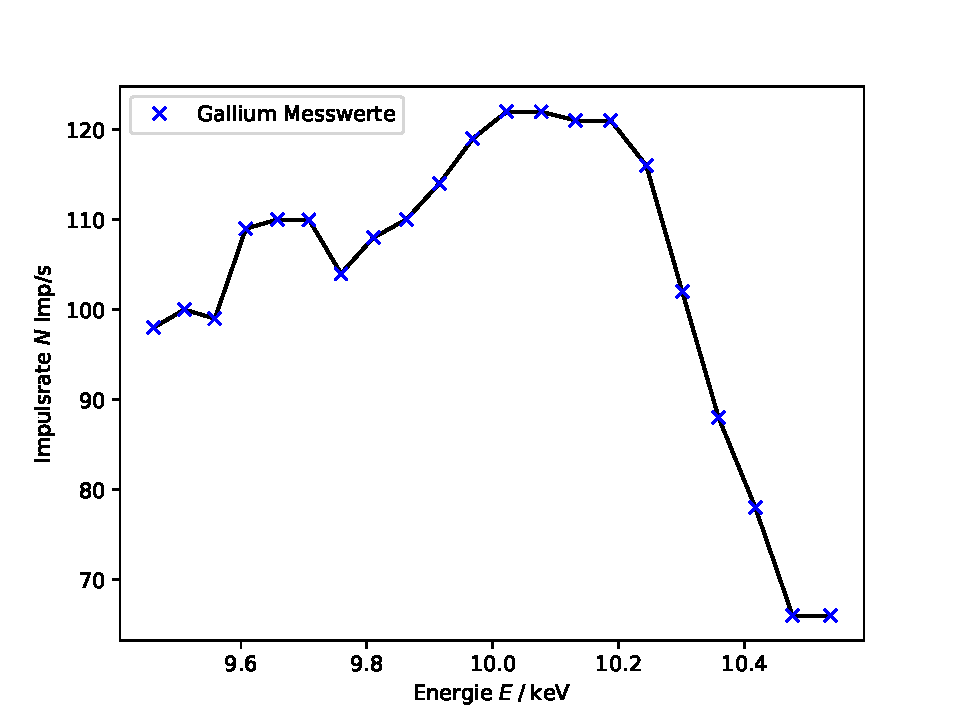
\includegraphics[width=0.7\textwidth]{plots/Gallium.pdf}
    \caption{In der Abbildung ist das Absorbtionspektrum eines Galliumabsorbers dargestellt}
\end{figure}
\begin{figure}[H]
    \centering
    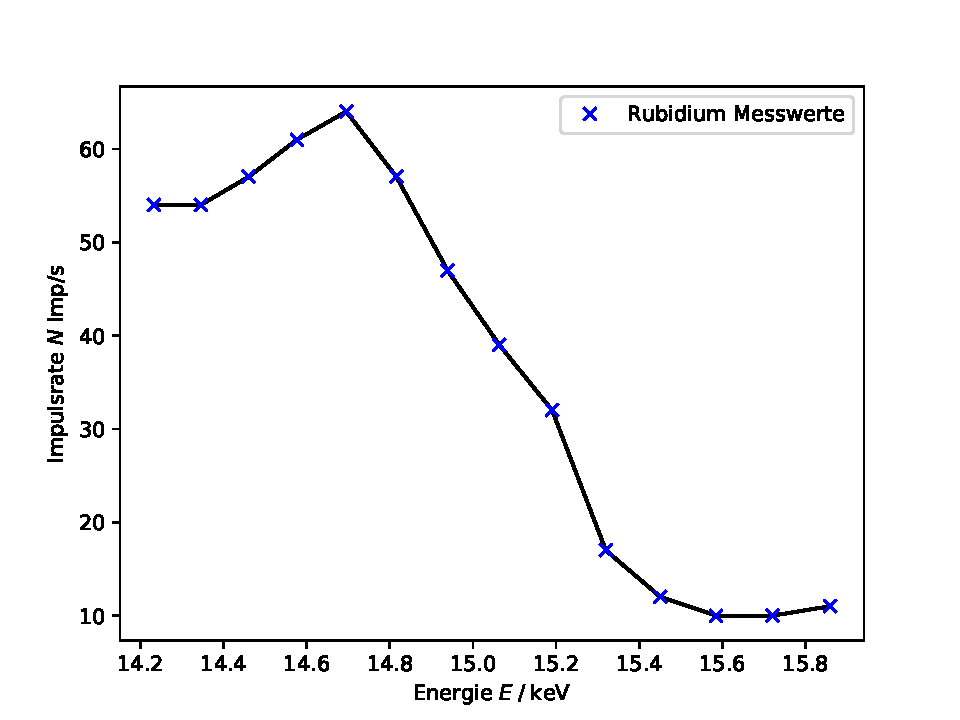
\includegraphics[width=0.7\textwidth]{plots/Rubidium.pdf}
    \caption{In der Abbildung ist das Absorbtionspektrum eines Rubidiumabsorbers dargestellt}
\end{figure}
\begin{figure}[H]
    \centering
    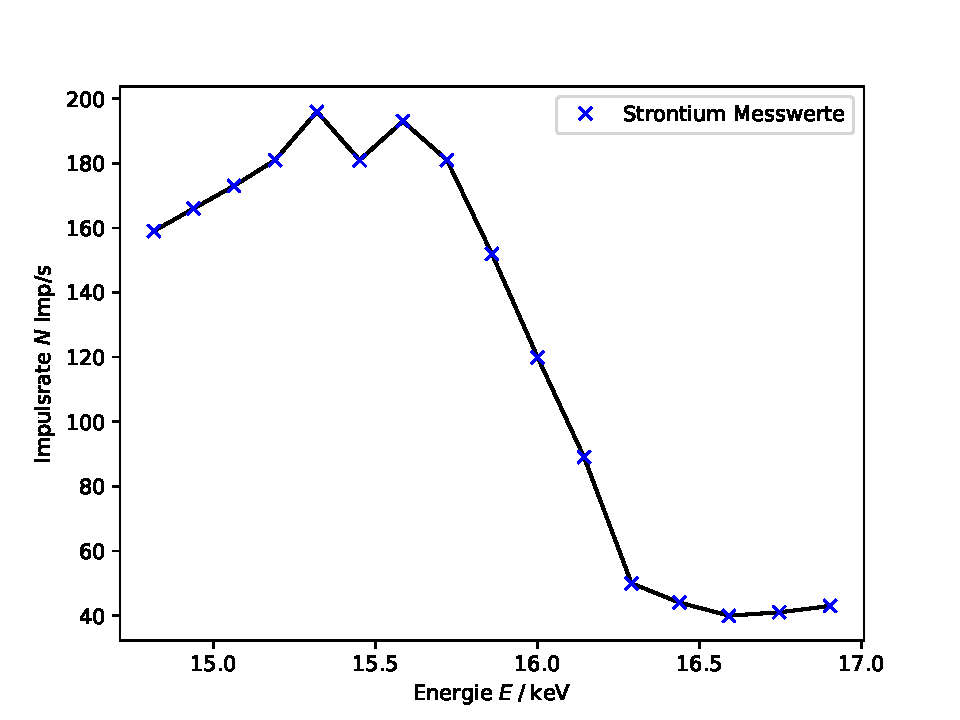
\includegraphics[width=0.7\textwidth]{plots/Strontium.pdf}
    \caption{In der Abbildung ist das Absorbtionspektrum eines Strontiumabsorbers dargestellt}
\end{figure}
\begin{figure}[H]
    \centering
    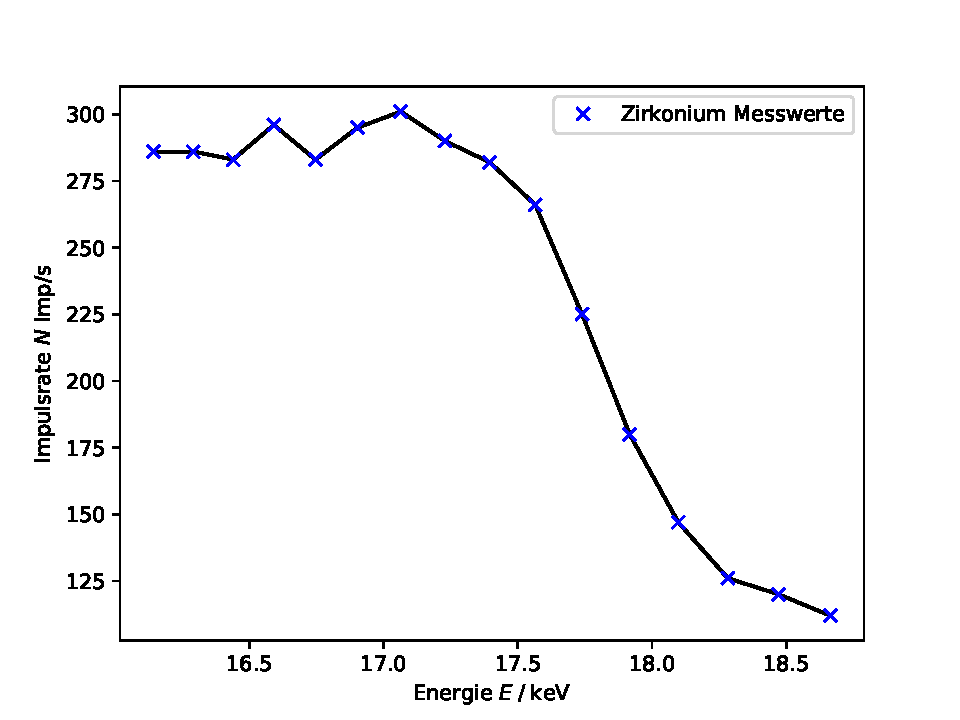
\includegraphics[width=0.7\textwidth]{plots/Zirkonium.pdf}
    \caption{In der Abbildung ist das Absorbtionspektrum eines Zirkoniumabsorbers dargestellt}
\end{figure}
\label{subsec:anhang1}
\subsection{Messwerte}
\begin{table}[H]
    \centering
    \begin{tabular}{c c}
        \toprule
        $\Theta\;/\;°$& $N\;/\;\frac{Imp}{s}$\\
        \midrule
        12.8&	10.0\\
        12.9&	12.0\\
        13.0&	9.0\\
        13.1&	13.0\\
        13.2&	18.0\\
        13.3&	21.0\\
        13.4&	25.0\\
        13.5&	27.0\\
        13.6&	27.0\\
        13.7&	22.0\\
        13.8&	25.0\\
        13.9&	21.0\\
        14.0&	23.0\\
        14.1&	20.0\\
        14.2&	21.0\\
        14.3&	19.0\\
        \bottomrule
    \end{tabular}
    \caption{Messwerte zum Absorptionsspektrum von Brom bei einer Beschleunigungsspannung 
    $U=350$kV und einem Strom von $I=1$mA.\\
    Gemessen wurde der Bragg-Winkel $\Theta$ und die Impulsrate $N$ mit einer Integrationszeit
    von $t=20$s pro Winkel.}
\end{table}
\begin{table}[H]
    \centering
    \begin{tabular}{c c}
        \toprule
        $\Theta\;/\;°$& $N\;/\;\frac{Imp}{s}$\\
        \midrule
        18.0&    58.0\\
        18.1&    54.0\\
        18.2&    55.0\\
        18.3&    54.0\\
        18.4&    54.0\\
        18.5&    55.0\\
        18.6&    65.0\\
        18.7&    84.0\\
        18.8&    91.0\\
        18.9&    100.0\\
        19.0&    102.0\\
        19.1&    100.0\\
        19.2&    98.0\\
        19.3&   100.0\\
        19.4&    95.0\\
        19.5&    98.0\\
        \bottomrule
    \end{tabular}
    \caption{Messwerte zum Absorptionsspektrum von Zink bei einer Beschleunigungsspannung 
    $U=350$kV und einem Strom von $I=1$mA.\\
    Gemessen wurde der Bragg-Winkel $\Theta$ und die Impulsrate $N$ mit einer Integrationszeit
    von $t=20$s pro Winkel.}
\end{table}
\begin{table}[H]
    \centering
    \begin{tabular}{c c}
        \toprule
        $\Theta\;/\;°$& $N\;/\;\frac{Imp}{s}$\\
        \midrule
        17.0&    66.0\\
        17.1&    66.0\\
        17.2&    78.0\\
        17.3&    88.0\\
        17.4&    102.0\\
        17.5&    116.0\\
        17.6&    121.0\\
        17.7&    121.0\\
        17.8&    122.0\\
        17.9&    122.0\\
        18.0&    119.0\\
        18.1&    114.0\\
        18.2&    110.0\\
        18.3&    108.0\\
        18.4&    104.0\\
        18.5&    110.0\\
        18.6&    110.0\\
        18.7&    109.0\\
        18.8&    99.0\\
        18.9&    100.0\\
        19.0&    98.0\\
        \bottomrule
    \end{tabular}
    \caption{Messwerte zum Absorptionsspektrum von Gallium bei einer Beschleunigungsspannung 
    $U=350$kV und einem Strom von $I=1$mA.\\
    Gemessen wurde der Bragg-Winkel $\Theta$ und die Impulsrate $N$ mit einer Integrationszeit
    von $t=20$s pro Winkel.}
\end{table}
\begin{table}[H]
    \centering
    \begin{tabular}{c c}
        \toprule
        $\Theta\;/\;°$& $N\;/\;\frac{Imp}{s}$\\
        \midrule
        19.5	&112.0\\
        9.6	    &120.0\\
        9.7	    &126.0\\
        9.8	    &147.0\\
        9.9	    &180.0\\
        10.0	&225.0\\
        10.1	&266.0\\
        10.2	&282.0\\
        10.3	&290.0\\
        10.4	&301.0\\
        10.5	&295.0\\
        10.6	&283.0\\
        10.7	&296.0\\
        10.8	&283.0\\
        10.9	&286.0\\
        11.0	&286.0\\
        \bottomrule
    \end{tabular}
    \caption{Messwerte zum Absorptionsspektrum von Zirkonium bei einer Beschleunigungsspannung 
    $U=350$kV und einem Strom von $I=1$mA.\\
    Gemessen wurde der Bragg-Winkel $\Theta$ und die Impulsrate $N$ mit einer Integrationszeit
    von $t=20$s pro Winkel.}
\end{table}
\begin{table}[H]
    \centering
    \begin{tabular}{c c}
        \toprule
        $\Theta\;/\;°$& $N\;/\;\frac{Imp}{s}$\\
        \midrule
        10.5&	43.0\\
        10.6&	41.0\\
        10.7&	40.0\\
        10.8&	44.0\\
        10.9&	50.0\\
        11.0&	89.0\\
        11.1&	120.0\\
        11.2&	152.0\\
        11.3&	181.0\\
        11.4&	193.0\\
        11.5&	181.0\\
        11.6&	196.0\\
        11.7&	181.0\\
        11.8&	173.0\\
        11.9&	166.0\\
        12.0&	159.0\\
        \bottomrule
    \end{tabular}
    \caption{Messwerte zum Absorptionsspektrum von Strontium bei einer Beschleunigungsspannung 
    $U=350$kV und einem Strom von $I=1$mA.\\
    Gemessen wurde der Bragg-Winkel $\Theta$ und die Impulsrate $N$ mit einer Integrationszeit
    von $t=20$s pro Winkel.}
\end{table}
\begin{table}[H]
    \centering
    \begin{tabular}{c c}
        \toprule
        $\Theta\;/\;°$& $N\;/\;\frac{Imp}{s}$\\
        \midrule
        11.2&    11.0\\
        11.3&    10.0\\
        11.4&    10.0\\
        11.5&    12.0\\
        11.6&    17.0\\
        11.7&    32.0\\
        11.8&    39.0\\
        11.9&    47.0\\
        12.0&    57.0\\
        12.1&    64.0\\
        12.2&    61.0\\
        12.3&    57.0\\
        12.4&    54.0\\
        12.5&    54.0\\
        \bottomrule
    \end{tabular}
    \caption{Messwerte zum Absorptionsspektrum von Rubidium bei einer Beschleunigungsspannung 
    $U=350$kV und einem Strom von $I=1$mA.\\
    Gemessen wurde der Bragg-Winkel $\Theta$ und die Impulsrate $N$ mit einer Integrationszeit
    von $t=20$s pro Winkel.}
\end{table}

\label{sec:anhang}